\chapter{Findings (Analysis and Evaluation)}


\section{Statistical Analysis to Test the Classifiers}



\begin{table*}[t]
\caption {Confusion matrix results with supporting statistical measures and summative standard descriptive statistics for PoseNet fall detection system training data set.} \label{tab:PoseNet}
\resizebox{\textwidth}{!}{%
\begin{tabular}{|l|l|l|l|l|l|l|l|l|l|l|l|}
\hline
 & True Positive (\%) & True Negative (\%) & False Negative (\%) & False Positive (\%) & Accuracy & Precision & Sensitivity & Specificity & Error Rate & FPR & F-Score \\ \hline
Min & 2.993\% & 84.987\% & 1.503\% & 0.000\% & 94.111\% & 91.667\% & 61.429\% & 99.448\% & 1.503\% & 0.000\% & 75.605\% \\ \hline
Max & 9.125\% & 95.179\% & 5.729\% & 0.509\% & 98.497\% & 100.000\% & 73.239\% & 100.000\% & 5.889\% & 0.552\% & 84.553\% \\ \hline
Mean & 5.096\% & 92.069\% & 2.723\% & 0.113\% & 97.164\% & 98.386\% & 65.847\% & 99.877\% & 2.836\% & 0.123\% & 78.774\% \\ \hline
Median & 4.714\% & 92.598\% & 2.214\% & 0.042\% & 97.531\% & 99.920\% & 64.403\% & 99.957\% & 2.469\% & 0.044\% & 78.345\% \\ \hline
Std Dev & 1.912\% & 3.263\% & 1.377\% & 0.174\% & 1.386\% & 2.900\% & 4.485\% & 0.190\% & 1.386\% & 0.190\% & 2.856\% \\ \hline
\end{tabular}%
}
\end{table*}





\begin{table*}[t]
\caption {Confusion matrix results with supporting statistical measures and summative standard descriptive statistics for OpenPose fall detection system training data set. } \label{tab:OpenPose}
\resizebox{\textwidth}{!}{%
\begin{tabular}{|l|l|l|l|l|l|l|l|l|l|l|l|}
\hline
 & True Positive (\%) & True Negative (\%) & False Negative (\%) & False Positive (\%) & Accuracy & Precision & Sensitivity & Specificity & Error Rate & FPR & F-Score \\ \hline
Min & 0.542\% & 93.345\% & 1.080\% & 0.000\% & 93.887\% & 75.309\% & 8.233\% & 99.807\% & 1.136\% & 0.000\% & 15.060\% \\ \hline
Max & 1.049\% & 98.313\% & 6.040\% & 0.188\% & 98.864\% & 100.000\% & 39.396\% & 100.000\% & 6.113\% & 0.193\% & 56.524\% \\ \hline
Mean & 0.701\% & 96.737\% & 2.519\% & 0.042\% & 97.439\% & 93.957\% & 24.768\% & 99.957\% & 2.562\% & 0.044\% & 38.464\% \\ \hline
Median & 0.686\% & 97.151\% & 2.133\% & 0.010\% & 97.773\% & 98.718\% & 23.493\% & 99.990\% & 2.227\% & 0.010\% & 38.046\% \\ \hline
Std Dev & 0.168\% & 1.463\% & 1.506\% & 0.065\% & 1.517\% & 8.862\% & 9.291\% & 0.067\% & 1.517\% & 0.067\% & 12.249\% \\ \hline
\end{tabular}%
}
\end{table*}

This section presents the statistical analysis that was performed to test the effectiveness of the classifier. Numerous confusion matrix computations were performed including supporting statistical measures and summative standard descriptive statistics. The confusion matrices show the range of values (min, max, mean, median and standard deviation) across all participants. These computational results are shown in Table 1 and Table 2 based on models created from training data sets.

% \begin{table*}[t]
% \resizebox{\textwidth}{!}{%
% \begin{tabular}{llllllllllll}
%  & True Positive (\%) & True Negative (\%) & False Negative (\%) & False Positive (\%) & Accuracy & Precision & Sensitivity & Specificity & Error Rate & FPR & F-Score \\
% Min & 2.993\% & 84.987\% & 1.503\% & 0.000\% & 94.111\% & 91.667\% & 61.429\% & 99.448\% & 1.503\% & 0.000\% & 75.605\% \\
% Max & 9.125\% & 95.179\% & 5.729\% & 0.509\% & 98.497\% & 100.000\% & 73.239\% & 100.000\% & 5.889\% & 0.552\% & 84.553\% \\
% Mean & 5.096\% & 92.069\% & 2.723\% & 0.113\% & 97.164\% & 98.386\% & 65.847\% & 99.877\% & 2.836\% & 0.123\% & 78.774\% \\
% Median & 4.714\% & 92.598\% & 2.214\% & 0.042\% & 97.531\% & 99.920\% & 64.403\% & 99.957\% & 2.469\% & 0.044\% & 78.345\% \\
% Std Dev & 1.912\% & 3.263\% & 1.377\% & 0.174\% & 1.386\% & 2.900\% & 4.485\% & 0.190\% & 1.386\% & 0.190\% & 2.856\%
% \end{tabular}%
% }
% \end{table*}


% \begin{figure}
%   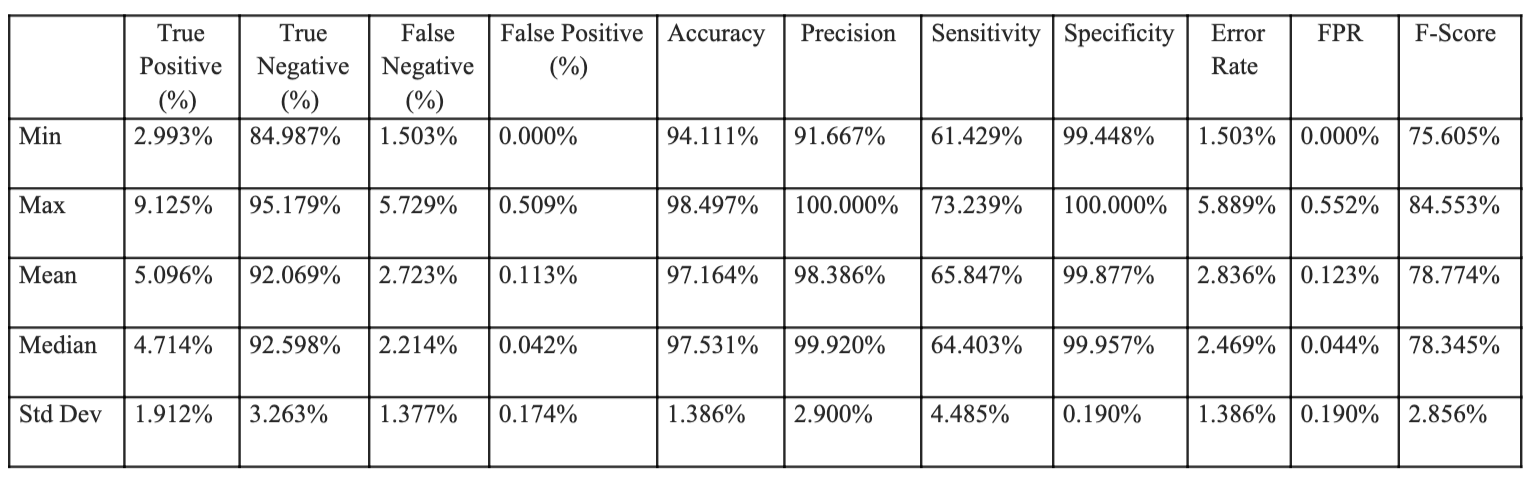
\includegraphics[width=\linewidth]{posenetTable}
%   \caption{Confusion matrix results with supporting statistical measures and summative standard descriptive statistics for PoseNet fall detection system training data set.}
%   \label{fig:posenetTable}
% \end{figure}



For our implementation using PoseNet, as shown in Table 1, on average 5.096\% of results were true positives, 92.069\% true negatives, 2.723\% false negatives, and 0.113\% false positives. The system exhibited a mean accuracy of 97.164\%, precision of 98.386\%, sensitivity of 65.847\%, specificity of 99.877\%, error rate of 2.836\%, false positive rate of 0.123\%, and a F-score of 78.774\%.


On our other fall detection system using OpenPose, Table 2 shows, on average 0.701\% of results were true positives, 96.737\% true negatives, 2.519\% false negatives, and 0.042\% false positives. The system exhibited a mean accuracy of 97.439\%, precision of 93.957\%, sensitivity of 24.768\%, specificity of 99.957\%, error rate of 2.562\%, false positive rate of 0.044\%, and a F-score of 38.464\%.


\section{Summary of Main Findings}

\begin{figure}
  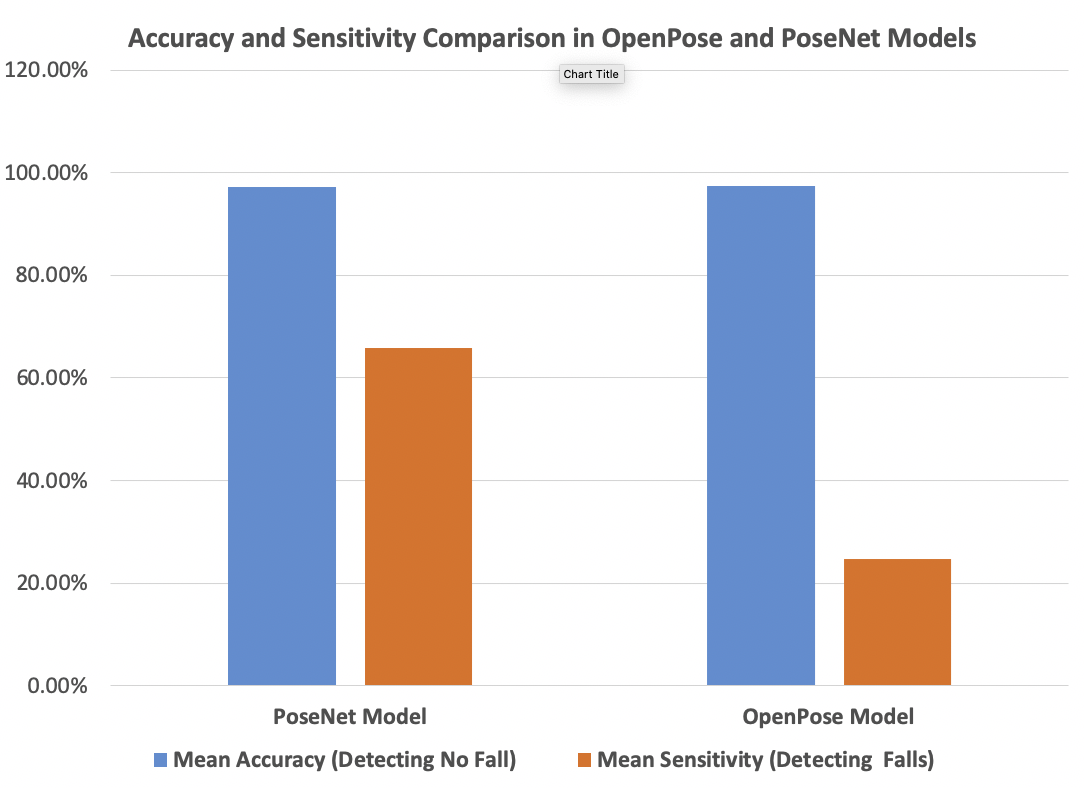
\includegraphics[width=\linewidth]{chart.png}
  \caption{Mean Accuracy and Sensitivity for PostNet and OpenPose Based Models.}
  \label{fig:chart}
\end{figure}


Figure ~\ref{fig:chart} shows a chart that compares the accuracy and the sensitivity of the two fall detection models. While both fall detection systems had a generally high accuracy at determining when someone wasn’t falling, as can be seen with the high true negative result and the high accuracy values of 97\% on both systems, along with the high specificity values of 99\%. As evidenced by the low sensitivity values of approximately 66\% on the PoseNet-based fall system and 25\% on the OpenPose-based fall system, actual fall detections will occur when they are supposed to, much less than 90\% of the time. The low standard deviation values across most variables also implies that these percentage values are relatively constant across the variety of datasets tested on, based on the nine participants in our experiment. While the accuracy was comparable in both models, the sensitivity was significantly less in the OpenPose implementation.




Figure ~\ref{fig:opsedetection} presents PoseNet and OpenPose keypoints superimposed over a frame of sample video.


\begin{figure}
  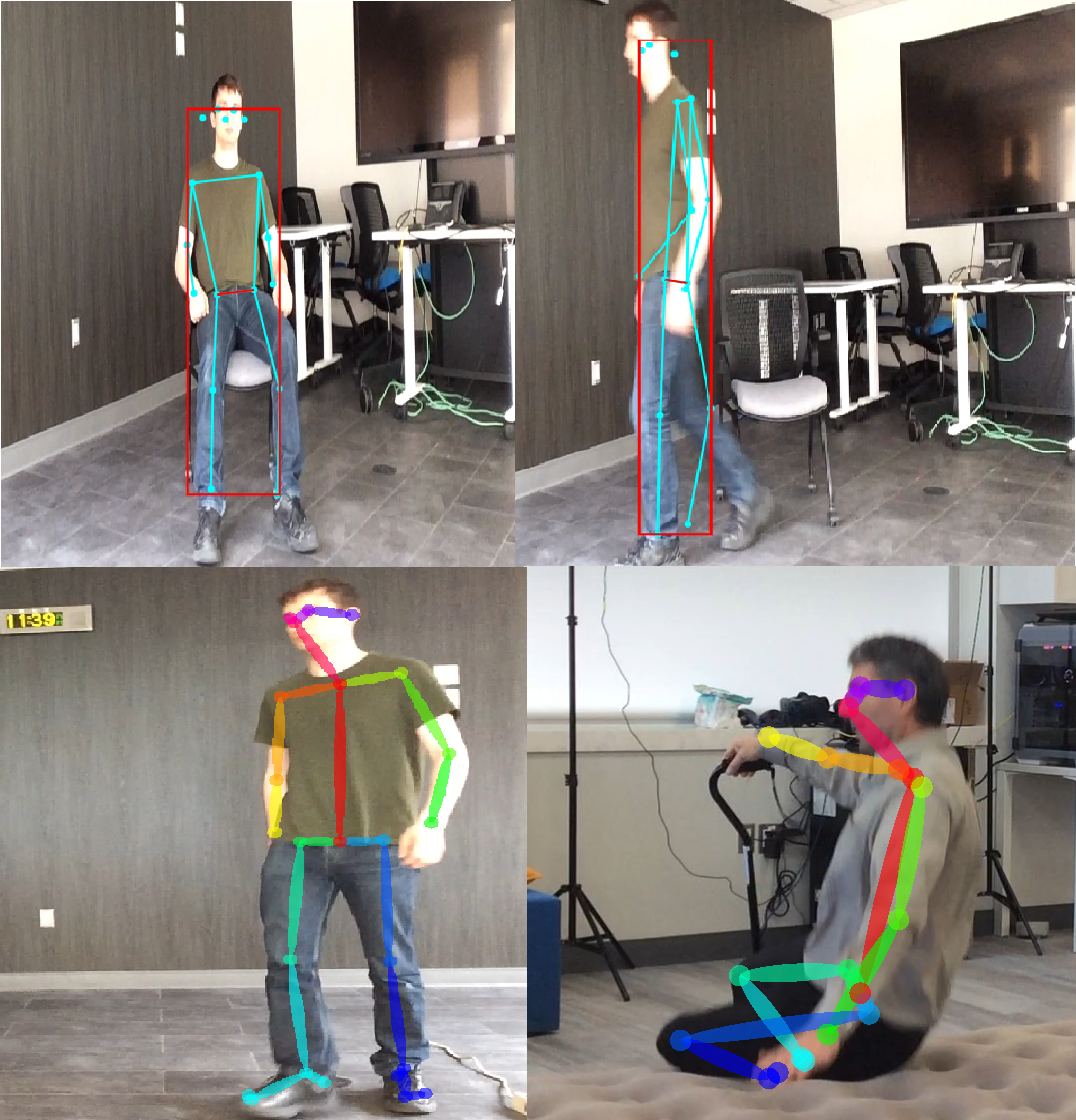
\includegraphics[width=0.7\textwidth]{opsedetection}
  \caption{PoseNet Pose Detection over Video (top) OpenPose Pose Detection over Video (bottom).}
  \label{fig:opsedetection}
\end{figure}





